\subsection{Resonance Magic Stick}\label{resonance-magic-stick}

This machine is to make anything with a spring or spring like thing or
pendulum vibrate. Vibration is generally part of the physical phenomenon
known as resonance, which I will discuss much more in the next volume.
For now suffice it to say anything you think of as a wave or vibration
is probably an example of some kind of resonance.

The way to drive pretty much any resonance is the same: push only when
your push is in the same direction as the natural motion from the
vibration. We do this with magnets, which both serve to create something
to drive against with the drive coils and also indicate motion direction
to the circuit which does the driving.

When electrical current goes through a wire in a magnetic field, there
is a force on that wire. The wire also creates a magnetic field, and we
can think of this system as an electromagnet(which we turn on and off
fast) and a permanent magnet(which is always on) either being pulled
together or pushed apart(either will work).

Detecting the motion of the magnet is done using induction: moving
magnetic fields generate voltage in a coil of wire, which we detect with
an amplifier. That amplifier is designed to be all or nothing: if there
is even a tiny voltage, it will go all the way to 5 volts(the power
supply voltage used in elementary Trash Magic as well as USB), and at
below that(including negative voltages) it's stuck at zero. What this
means is that it essentially detects the \emph{direction} of motion of
the magnet. Linking the output of that amplifier to a power switch(this
role is played by a type of transistor in the first version presented
here) which controls current through the drive coil(the coil that
actually drives the magnet) causes force to be applied to the magnet on
only one side of the cycle of motion.

Perhaps this is all confusing. It's just an electrical way of doing what
you do when you push someone else on a swing: you see when they are
going forward and push then. Thats' all we're doing! But with a pair of
electrical devices, one of which takes the place of your eyes watching
the moving swing(that's the amplifier) and one playing the role of your
hand pushing the swing(that's the transistor and drive circuit).

The drive coil is a coil of wire about 1-2 inches in diameter with
200-500 turns of wire. This is 30 AWG(American Wire Gauge) copper wire,
and it's a few dozen meters, which makes it a few ohms of resistance. At
5 volts, this means it's generally 0.5 to 2 amps or so, that's the
target. The sense coil is 50 turns of the same wire, wrapped around the
outside of the drive coil.

\begin{figure}[htbp]
\centering
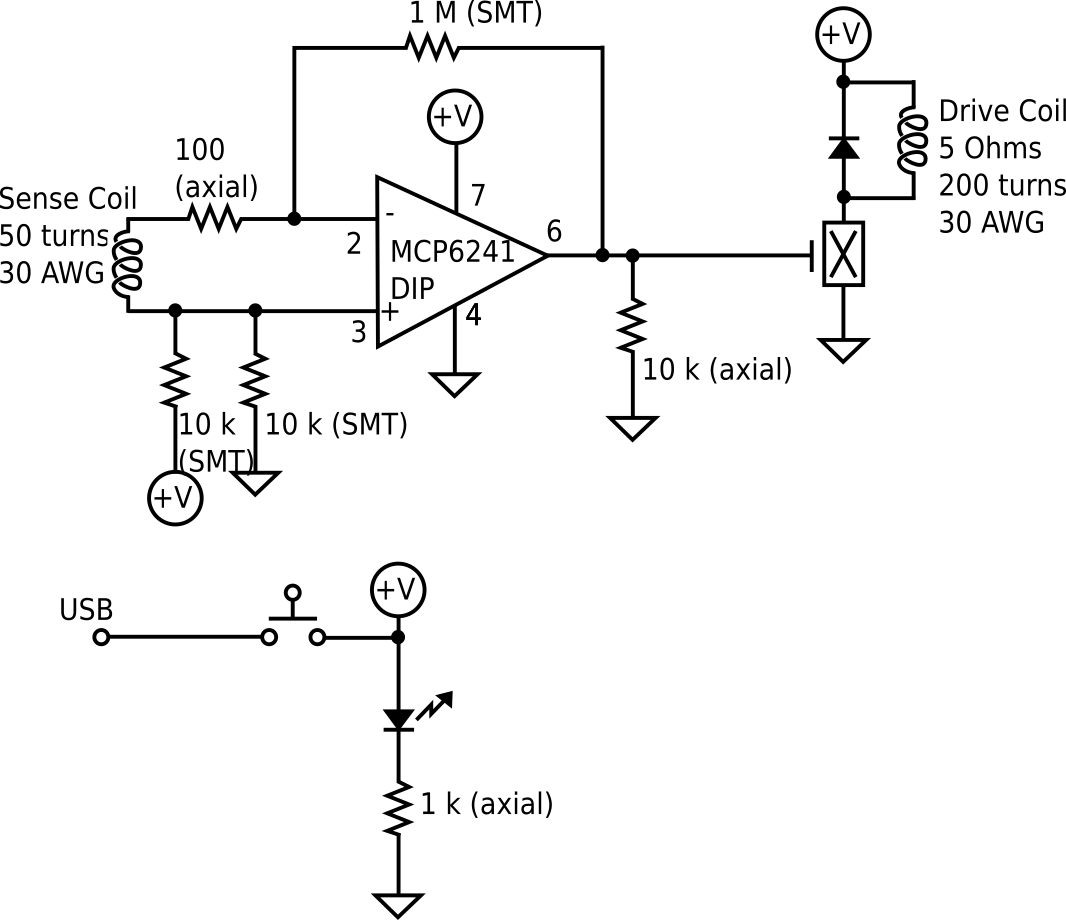
\includegraphics{images/resonantStick1.png}
\caption{Circuit schematic for resonant driver}
\end{figure}

The amplifier is a circuit using the MCP6241 operational amplifier, a
very low cost(less than a dollar), easy-to-use and generic chip from
Microchip, Inc.(also a very generic name!) The voltage gain is 10,000,
so 1 millivolt input is enough to saturate the amplifier all the way to
5 volts.

\begin{figure}[htbp]
\centering

\includegraphics{images/coilzoom.png}
\caption{Coil}
\end{figure}

\begin{figure}[htbp]
\centering

\includegraphics{images/bigoscillator.png}
\caption{stick}
\end{figure}

\begin{figure}[htbp]
\centering

\includegraphics{images/transistorimage.png}
\caption{transistor}
\end{figure}

\begin{figure}[htbp]
\centering

\includegraphics{images/ampimage.png}
\caption{amp}
\end{figure}

A core of ferromagnetic material such as steel ball bearings filled into
JB weld steel epoxy can increase the inductance considerably, and also
making it possible to drive steel or iron objects without permanent
magnets.

The strobe light is a high power small LED flashlight driven through
another identical power transistor, controlled by the output of a 555 in
monostable mode driven by the output of the amplifier. The user can turn
a knob that is a potentiometer that controls the time delay, generally
some number of ms or 10's of ms or 100's of ms. This strobe is thus
perfectly timed with whatever the resonant frequency is, and varying the
time delay varies what phase of that wave we can see.

The combination of a wave drive and a strobe has many applications in
both science and art. A wave tank can be made which projects water waves
in a shallow clear dish onto a large screen(2 m across), and waves can
be generated using the vibrational drive and a small agitator of some
kind(a wood stick or blunt wire will work). This can be an interesting
art piece that allows you to observe wave behavior with the strobe. Is
it art or science? Both. Also the strobe can be used in microscopy with
vibrating water, and the \emph{observed} position of a floating object
in the fluid can be controlled using the phase knob! This can be
extended into a whole world of optical microscopy, as well as other
phase controlled measurements in a vibrating fluid.

A phase controlled standing wave illumination can be used to make living
art by growing tiny plants in large arrays in such light, and
controlling the phase to control the relative illumination across the
green surface, making waves in the living plants. Many different art
pieces could be made like this, including growing bansai trees with this
illumination over a many year period to make trees with standing waves
of vibrational motion and light.

Art can also be constructed by making the strobe illuminate various
interesting steel objects which vibrate. This can also be used for pure
light art with more LEDs on the steel.

Vibrational drive can also be an alternative to rotational drive for
tools to work stone and wood. A coil with a iron core can be used to
pull on an iron nail on a spring, which then vibrates along the long
axis of the nail, making a sort of small steel jackhammer. Used under
water with patience and some automation, this could be a tool to slowly
and safely chip away at stone to make arbitrary shapes with minimal
energy or time or effort input. The same technology can of course be
used for wood.

Vibrational oscillators can also have a variety of applications in
massage and health, both for humans and other animals. Vibration applied
to various compost reactors and other types of chemical and biological
reactors can make a simple method for mixing or increasing reaction
rates. What effect does vibration have on microorganisms in loose soil?
Is it ever good? We must study this and find out.

Another simple vibrational machine that our driver can drive is a
pendulum with full swing. This can be as simple as a stick with a hole
in it and a metal rod as axle running through a plastic bottle stator,
with magnets on the ends of the stick. The driver will periodically
drive the magnets with just the right frequency and phase using feedback
as with the linear oscillator. This leads to an accelerating rotational
motor limited by the friction of the bearings, which has several
applications. One of the most useful is the high voltage generator,
where the rotation causes a rubbing between two materials that built up
voltage, and then metal pickups transfer charge to a big metal ball and
thousands of volts are built up which can be used for various things
such as plasma physics. These types of rotational pendulums are also a
nice demonstration of Josephson Junction physics and can be useful for
building models for that field of research.

Vibrational machines can also be used for simple propulsion of robots
and for pumps of both fluids and gasses. It is also amusing to see how
destructive resonance can be by putting magnets on glass things and
smashing them with the driver, which should be done very carefully if at
all!

\subsection{Noise Magic Stick}\label{noise-magic-stick}

This stick allows us to both listen to and create noise magic. Noise
magic has many forms, and we will work with several. First of all this
will be designed to measure the noise in tiny magnetic fields, amplify
it, and make audio noise for the human ear. This means you can literally
hear magnetic fields, and by brandishing your magic stick you can
control very sensitively what fields you're listening to: changing
direction with a tiny twist of the stick and location by waving it
around your head.

Two stages of high gain amplifier and one stage of buffer amplifier get
from the detection coil to the speaker. All amplifiers and the speaker
are powered by a 5V source from any USB type supply and like the
Resonant Stick the input will be a USB cable. The top of the stick is
the speaker and the bottom is the pickup coil, with many turns and a
ferrous core. Potentiometers are used to tune so that all signals are
centered in the middle between 0V and 5V. This then goes through a
isolator to the last stage to let all AC through but not any DC into the
speaker. Large, obviously labelled, wires connect to the feedback
resistors in the gain stages, making it easy to make summing or
differentiating amps as well as oscillators. Magnets can be used to
couple vibration to electricity to sound, for direct vibrational
amplification. Knobs and switches can thus choose gain, keep DC at zero,
and make musical effects for art.

In the highest gain mode with a resistor at the input the stick can be
used to measure thermal noise of the resistor. This can be repeated for
various fluids, making a Johnson noise detector of fluid impedance which
should also be sensitive to drift currents from whatever is going on
electrically in the fluid. In addition to thermal noise there will be
shot noise observable from quantum tunneling through various native
oxide layers. This can be accomplished with an old beer can found by the
creek, immersed in a sports drink. Direct interaction with the
properties of the oxide using acoustic feedback should thus be possible
using quantum tunneling noise.

Properly wielded and modified, the Noise Magic Stick should be our ears
into a vast world of electrical impedance, voltage, current, and ion
magic in general. This is a precursor tool to the generic
electrochemical probe that will be made in Volume II of this work.
Again, with practice, it should be possible to do physical measurements
on arbitrary materials using the Stick, both electric and magnetic.

Another extremely important mode of operation for the Noise Magic Stick
is for optical pickup. A very simple and cheap optical sensor can be
connected to the input of the amplifier chain, converting an optical
signal to an audio signal. This can be used to demodulate voice signals
sent using fire and smoke and vibration in a faraway location. Optics
can be built into the stick to focus on a specific point, which might be
a transmission fire far away. Another magician may thus transmit via one
fire on a mountain top and be picked up and amplified as a loud acoustic
signal by many other magicians miles away in different locations! This
can also be done with fluids and at the microscopic scale with different
optics to create an audio signal from a microscopic system, generally a
biological one. We can thus listen to the motion of the cilia on a
moving protozoan for instance as an actual audio signal. This is both
art and science and also technology.

Finally Noise Magic gives us another useful resource: truly random
numbers. Using physical noise like thermal or shot noise we can have a
signal which is physically provably random which can generate numbers
using a simple analog to digital converter and microprocessor, at least
for now. In the future, the better way to do this would be to have the
random bits get directly encoded into something physical in multiple
copies which can then be used for a physical one time pad with no
interaction with any microprocessor ever. We can thus have provably
secure communication based on face to face contact, which can then be
deployed over any distance using the trivial one time pad encryption.
The attacks against the one time pad key generation generally involve
compromising the hardware in ways that involve access to the industrial
process by which that hardware was made. We make our own hardware as art
built from trash and then distribute it face to face, so these problems
to not apply. I don't generally believe in the cypher punk world view,
but near-theoretically-perfect encryption can be useful and it should be
so easy with our system there is not reason not to do it.

\subsection{Whirligig}\label{whirligig}

Whirligig and charger: - all kinds of stick pendulums that just spin
around for a long time - just a simple whirligig that runs forever as an
undershot water wheel - small bucket overshot whirligig that does
nothing but spin - generator that charges 5 V capacitor with any
magnetic induction with either sign - magnet rotor with stick bearing
and big iron core pickup connected to generator - whirligig that runs a
light and that's all - whirligig that charges USB - rooftop wind
whirligig that charges USB

\subsection{Lesson Gifts}\label{lesson-gifts}

My problem is the same as that of Kano in forming the Kodokan: how I
teach the first students and how I organize the information conveyed to
them shapes how they pass it on, and that will propagate through the
whole subsequent series of events. How did Kano start? How did Ueshiba?
Why was Kano able to build a more functional system than Ueshiba?

We must encourage collaboration so that those who don't want to learn
electronics can get free electronics from those who do, and can find
other ways to contribute, with art, assembly, craft, and the important
courier service that needs to happen for distribution.

\subsection{Courrier Gifts}\label{courrier-gifts}

Recruiting couriers might be the most important of these construction
tasks, as I will be always building more artifacts myself and spreading
the teachings of how to do it face to face, which can't spread as fast
as the book can. The book can spread \emph{very} fast, and build a
courier network so that physical artifacts can also if the book spreads
the courier network very fast(it should also explicitly encourage
readers to spread the word fast), and I can make artifacts fast, the
limiting factor in growth will be the spread of the craft of artifact
creating and the use of the new things.

\subsection{Version 1 of Tale and
Lore}\label{version-1-of-tale-and-lore}

\subsection{Deploy Guerrilla Faery
Art}\label{deploy-guerrilla-faery-art}

how to do installations, how to fix them how to document them, how to
expand them how to move them, documentation of installations around the
world, USB chargers are best to start with

from the blog:

I have figured out the nature of the first phase of technology
development: guerilla faery art. I've been getting distracted by the
long term goals of functionality for industrial production, but for this
first volume aimed at non technical readers, it makes sense to focus on
technology which will make sense and be obviously worth spreading:
guerilla faery art. What is this? Art outside the capitalist system,
installed without permission, built from trash and powered from freely
available energy, and with a view toward exposing people to the of magic
of the physical world. There will be oscillators and motors and pumps
and strobe lights and magnetic pickups and all kinds of blinking lights
and speakers for sound and microscopic views of living things.

The electrochemical probe and full robotic system belongs to the second
volume on Trash Magic. That is geared to people who want to delve deeply
into the way electromagnetic trash magic works, focusing on fluid ion
transport to interact with living systems, along with the basic
infrastructure needed for a good life. The more advanced stuff will be
just described in the first volume, not built out with detailed plans.

What does this mean for things to build?

Materials and how to mount things in place matter. This gives me an
excuse to go down to all the creeks and find the right sticks and rocks
and trash locally that can be repurposed for an installation. Some
missions will require stealth.

Viewing of microscopic objects must be extremely robust and require no
turning on or off or care on a day to day basis. Obviousness is key
here, the view port has to be so obvious that everyone will
automatically use it. Also the subject has to naturally flow in
constantly, with some trickle from a living stream so that something
interesting, whatever the subject is, is usually present.

What specifically needs to get built to have finished products, and
where do they go? Some things will be deployed in wild areas, some in
urban areas, and some will be gifts to artists.

A tentative and partial list of Guerilla Faery Art:

\begin{itemize}
\tightlist
\item
  USB charger with water wheel
\item
  water wheel that generates electricity which drives oscillator stick
  with rocks on it, just vibrates forever with feedback
\item
  same, but with LEDs with a pattern to make 3d POV art in the water
\item
  water wheel turns triboelectric generator using bottles and such to
  build up high voltage which creates an arc over the water between
  aluminum covered plastic bottles, very visible at night!
\item
  art piece as gift where a vibrator vibrates water, making waves, which
  can be observed using a strobe, and turned into audio with a magnetic
  float and amplified magnetic pickup. With the magnifier built into the
  wood/plastic/stone water containers, this connects the main
  technologies if it's USB powered, and is the perfect Main Gift for
  this phase.
\item
  3d manipulator with 3d input, hung from a tree or bridge over the
  water, which powers all motors and control circuits. Anyone happening
  by and seeing the setup can grab the input rock and move it around,
  which will drive the moving platform around in 3d space above the
  water. This probe can have the crude sonic electrochemical probe tuned
  to respond to depth in the water, so that the user can make sound by
  controlling the probe around in the water. Here art, science and
  technology are all one thing, built from trash, and in a public place
  with no declared ownership.
\item
  water channel with strobe and vibrational drive for visual effects at
  night, driven by water wheel, runs all the time
\item
  evaporative cooling refrigerator driven by water wheel
\item
  hotplate driven by water wheel
\item
  warm water pool heated by water wheel and generator
\item
  steam powered organ using tubes and steam generated from water wheel
\item
  datalog of creek which can connect to phones and twitter
\end{itemize}

Focusing on the main thing for now it's probably the USB driven art
piece without the generator, just a wall charge for a off the shelf lipo
battery, or left plugged in. A wave tank with a strobe can have a
tunable 2d shape projected by the sun down onto an area, with musical
output based on the wave patterns. This could be installed in a tree,
projecting through glass, with water piped from the top of a waterfall.
But what powers it? No, I need the charger for the guerilla
installation, but not for the art gift.

Art gift should be simpler than that, project up and along the side,
with lights under transluscent plastic in the stick. Vibrator stick with
rocks on it bounces, with a stick that can be adjusted to agitate the
water with different wave shapes and frequencies and amplitudes. The
magnets and rocks can also be moved to change the properties. Water
propagates down carved channels in a fat bottom stick with the drive
stick bolted to it as well as the bouncing stick which is fixed at the
end opposite the water. Lenses can be put above the water to magnify
what is in it as well as to project light in various directions both for
art and for observation. A little wave pool at the opposite end of the
water agitator has a float with a tiny magnet in it, and the audio flux
amplifier is wound around this pool, so that the sound is picked up and
amplified and has an audio out socket. A beautiful carved wooden knob is
used to adjust the strobe properties by changing a 555 circuit.

This is the first thing! Build this art gift first, before the water
wheel, it's self contained and can be distributed and used in classes I
can teach and spread the work. Lack of water wheel is not serious for
most people since they charge devices anyway with USB and can get a lipo
at a gas station for 10 dollars.

\subsection{Future Work}\label{future-work}

I will list the things I'll leave for other projects/publications:

\begin{enumerate}
\def\labelenumi{\arabic{enumi}.}
\tightlist
\item
  robots that roll around
\item
  3d input manipulator
\item
  3d probe
\item
  stepper motor
\item
  water powered drill
\item
  microscopy
\item
  fluidic pumps
\item
  cable to move goods around mechanically driven by whirligig
\item
  water pump driven by water
\item
  generic air pump for inflating anything, which is also generic water
  pump
\item
  electrostatic generator driven by whirligig
\item
  stone cutting machine
\item
  boat
\item
  heated composting reactor
\item
  oxygen and hydrogen generator
\item
  electrochemical probe
\item
  optical free space communications system
\item
  soaring high voltage drones
\item
  temperature regulator using stepper motor and solar concentrator with
  parabolic mirror from trash
\item
  thermometers
\end{enumerate}

\begin{itemize}
\tightlist
\item
  how to make a thing
\item
  how to ship a thing
\item
  how you can get finished goods and join a value circle
\item
  how you can make stuff and start a value circle
\item
  how you can do a research project and start a value circle
\item
  how to transport a thing from the maker to the user
\item
  how to find your ambient energy resources
\item
  what you can do to spread the word and build community
\item
  Other academic work you can contribute as a scholar
\item
  Machines you could build outside this system which can start a new
  value circle
\end{itemize}

This section should have some basic assembly plans and information to
get started even without the second volume.

Things to make here:

\begin{itemize}
\tightlist
\item
  vibrational oscillator with musical pickup
\item
  3d input device
\item
  3d manipulator, linked to input device
\item
  wood cutting for circuits techniques
\item
  plastic welding techniques
\item
  waterwheel generator to 5V USB charger
\item
  skeletron guide, with pictures, cartoons, detailed instructions,
  several plans:

  \begin{itemize}
  \tightlist
  \item
    tent
  \item
    water wheel
  \item
    tripod for manipulator and probe
  \item
    vibrational musical instrument
  \item
    boat
  \end{itemize}
\item
  high voltage generator
\item
  strobe microscope
\item
  LED art vibrator display
\item
  basic electrochemical probe
\item
  temperature regulator with hoist and thermometer and fire
\item
  ambient art pieces powered off water and wind that use electricity to
  do things which can be repaired forever by anyone and moved and
  rebuilt and replaced by anyone
\item
  vibrator with polished stones as massager
\item
  Josephson junction pendulum
\item
  build a heated shit reactor with a giant tube and air pump to send
  gasses to the top of a tree
\end{itemize}
